\documentclass[10pt]{article}
\PassOptionsToPackage{hyphens}{url}
\usepackage{hyperref}
\usepackage[margin=0.75in]{geometry}

\usepackage{multicol}
\usepackage{textcomp}
\usepackage{color}
\usepackage{graphicx}
\definecolor{pblue}{rgb}{0.13,0.13,1}
\definecolor{pgreen}{rgb}{0,0.5,0}
\definecolor{pred}{rgb}{0.9,0,0}
\definecolor{pgrey}{rgb}{0.46,0.45,0.48}

\usepackage{listings}
\lstdefinestyle{term}{language=bash,
  columns=fullflexible,
  showspaces=false,
  showtabs=false,
  breaklines=true,
  showstringspaces=false,
  tabsize=2,
  breakatwhitespace=true,
  commentstyle=\color{pgreen},
  keywordstyle=\color{pblue},
  stringstyle=\color{pred},
  basicstyle=\small\ttfamily,
  frame=single,
  moredelim=[il][\textcolor{pgrey}]{$$},
  moredelim=[is][\textcolor{pgrey}]{\%\%}{\%\%},
  upquote=true
}
\lstdefinestyle{sh}{language=bash,
  columns=fullflexible,
  showspaces=false,
  showtabs=false,
  breaklines=true,
  showstringspaces=false,
  tabsize=2,
  breakatwhitespace=true,
  commentstyle=\color{pgreen},
  keywordstyle=\color{pblue},
  stringstyle=\color{pred},
  numbers=left,
  stepnumber=1,
  basicstyle=\small\ttfamily,
  frame=single,
  moredelim=[il][\textcolor{pgrey}]{$$},
  moredelim=[is][\textcolor{pgrey}]{\%\%}{\%\%},
  upquote=true
}

\lstdefinestyle{py}{language=python,
  columns=fullflexible,
  showspaces=false,
  showtabs=false,
  breaklines=true,
  showstringspaces=false,
  tabsize=2,
  breakatwhitespace=true,
  commentstyle=\color{pgreen},
  keywordstyle=\color{pblue},
  stringstyle=\color{pred},
  numbers=left,
  stepnumber=1,
  basicstyle=\small\ttfamily,
  frame=single,
  moredelim=[il][\textcolor{pgrey}]{$$},
  moredelim=[is][\textcolor{pgrey}]{\%\%}{\%\%},
  upquote=true
}

\lstdefinestyle{txt}{
  columns=fullflexible,
  showspaces=false,
  showtabs=false,
  breaklines=true,
  showstringspaces=false,
  tabsize=2,
  breakatwhitespace=true,
  numbers=left,
  stepnumber=1,
  basicstyle=\small\ttfamily,
  frame=single,
  moredelim=[il][\textcolor{pgrey}]{$$},
  moredelim=[is][\textcolor{pgrey}]{\%\%}{\%\%},
  upquote=true
}

\usepackage[T1]{fontenc}

\title{\textbf{Week 03} \\
ssh, grep, regexes, if, and bash scripts
}
\author{
	Melvyn Ian Drag
}
\date{\today}


\begin{document}
\maketitle

\begin{abstract}
Tonight we'll look at grep a bit more, we'll learn what a regex is, youll see
how if statements work in bash, we'll see a tidy way to write bash commands, and
you'll use a cool tool called ssh.
\end{abstract}

\section{ssh}
Let's start with the coolest thing. We'll make a remote connection to a remote
pc. At my house I have a raspberry pi running. 

{\LARGE \textbf{Now connect to the pc using ssh from the command line. And poke
around a bit. Class should think it's cool}}

Now I want you to do the same thing. To do this you need an ssh key. To get a
key you open git bash, a linux terminal or a mac terminal. Type `ssh-keygen' and
then just hit yes to everything. \textbf{Show the class how to do this using git
bash }. Then:

\begin{lstlisting}[style=term]
mel@laptop$ cd 
mel@laptop$ pwd
/home/mel/
mel@laptop$ ls -a
.. lots of stuff including a .ssh directory
mel@laptop$ cd .ssh
mel@laptop$ ls 
id_rsa id_rsa.pub
mel@laptop$ cat id_rsa.pub
A LOT OF STUFF
\end{lstlisting}

Now I want you to be able to connect to my raspberry pi

I need everyone to get me his or her id\_rsa.pub.

Actually have everyone email me the id\_rsa.pub file.


Then Im going to do some magic on my end and you'll be able to connect ot my
computer. We have alot to cover today so go fast, get this done, I don't want
this to take the whole class!

(Add the keys to the homeserver and then the students can connect to my
raspberry pi)

\begin{figure}[h]
\centering
	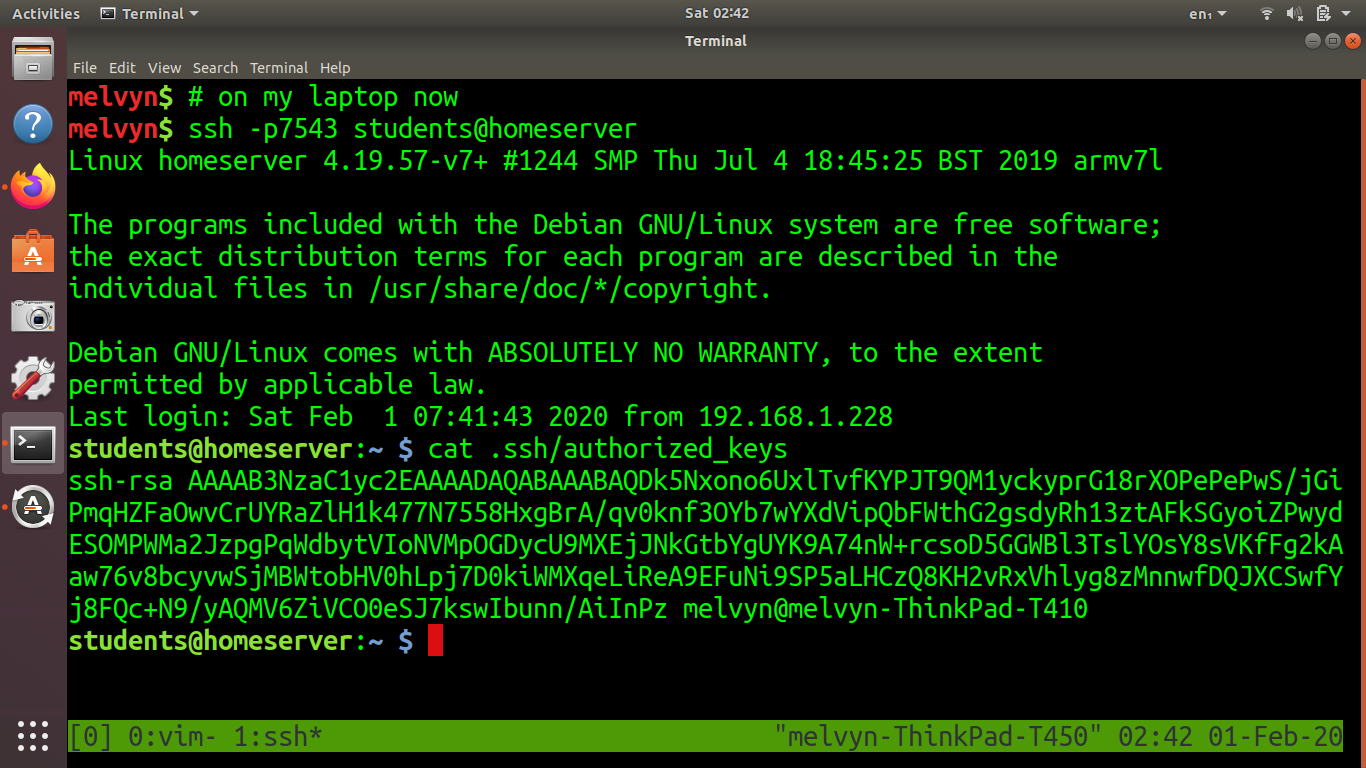
\includegraphics[width=0.8\textwidth]{Images/sshToHomeserver.png}
	\caption{I need to add your ssh key to my authorized\_keys file so you can
connect to my raspberry pi}
	\label{fig:firstssh}
\end{figure}


To connect you'll need to type

\begin{lstlisting}[style=term]
student@njcuPC$ ssh -p 7543 students@72.76.164.224
\end{lstlisting}

and then you should see your prompt change to 

\begin{lstlisting}[style=term]
students@homeserver$
\end{lstlisting}

you're now connected to a computer I have at home using a tool called ssh! There
are some commands that haven't worked in git bash yet like lsblk, wget and man
because those are linux only commands - if you try them now, you'll see they
work

{\LARGE WARNING! I don't know if my server can support 25 people logging in.
This might fail for some, or the computer might work painfyully slow. This is a
server I set up and didn't configure, I don't know what hte default params are.
you can limit the number of remote connections, and the raspberry pi is a small,
humble machine, it probably will cry when 25 ppl try to work on it
simultaneously. Let's see, I've never tried this before! Right now if you were a
hacker you would probably be able to do damage to me because I've allowed you
into my jome network, but I don't think anyone here knows enough yet to do me
any damage.}

Try downloading something with wget:

\begin{lstlisting}
student@homeserver$ wget
https://raw.githubusercontent.com/melvyniandrag/LinuxClassRepo/master/Lectures/Week03_SSHandMoreBash/a.txt

student@homeserver$ man cp
info about the cp command
student@homeserver lsblk
# some stuff about the drives on my rpi.
\end{lstlisting}

This is a turning point in your life if you've never done this before! I use ssh
almost every day, and so do many othe rprogrammers. Connecting to remote
computers is a very common, everyday thing you do. Especially if you are a
sysadmin or a webdev. A sysadmin needs to update computers reomtely - they use
ssh to connect to a far away computer nad then install stuff and log off.
Webdevs log onto webservers and then upload their website. We'll learn all this
later.

TAKE AWAY RIGHT NOW: You are connected to a linux computer in my apartment in
union City from a pc here in Jersey City. you could use this tool to connect to
a computer in China, or to connect to a computer on the international space
station. Nifty.

Please log off. I'm going to remove your keys and reboot the machine now, I
don't want you all mucking around on my home network.

{\LARGE Make sure to delete the keys and rebot the machine to make sure no one
can get on anymore}

For your homework you are oging to set up a digital ocean server. its a very
simple thing, but it might take you a few days. you have to go on the website
and put your .edu email and theyll give you a free linux coputer somewhere over
in clifton. You will use ssh to connect to this pc for the rest of the semester.

I'll get you a link where you go to get your free pass, its a 50 dollar credit
and then youll create a machine in the cloud and connect to it using ssh. No
more windows for us. And use the cloud machine even if you have a mac or ubuntu
laptop - there will be subtle differences that will be a pain i the neck for us.
Lets all just use a debian 10 server. Debian 10 is the operating system.



\end{document}
